%%%%%%%%%%%%%%%%%%%%%%%%%%%%%%%%%%%%%%%%%
% FRI Data Science_report LaTeX Template
% Version 1.0 (28/1/2020)
% 
% Jure Demšar (jure.demsar@fri.uni-lj.si)
%
% Based on MicromouseSymp article template by:
% Mathias Legrand (legrand.mathias@gmail.com) 
% With extensive modifications by:
% Antonio Valente (antonio.luis.valente@gmail.com)
%
% License:
% CC BY-NC-SA 3.0 (http://creativecommons.org/licenses/by-nc-sa/3.0/)
%
%%%%%%%%%%%%%%%%%%%%%%%%%%%%%%%%%%%%%%%%%


%----------------------------------------------------------------------------------------
%	PACKAGES AND OTHER DOCUMENT CONFIGURATIONS
%----------------------------------------------------------------------------------------
\documentclass[fleqn,moreauthors,10pt]{ds_report}
\usepackage[english]{babel}
\usepackage{float}
\usepackage{array}

\graphicspath{{fig/}}
\usepackage{subcaption}




%----------------------------------------------------------------------------------------
%	ARTICLE INFORMATION
%----------------------------------------------------------------------------------------

% Header
\JournalInfo{FRI Natural language processing course 2024}

% Interim or final report
\Archive{Project report} 
%\Archive{Final report} 

% Article title
\PaperTitle{Parameter-Efficient Fine-Tuning of Language Models} 

% Authors (student competitors) and their info
\Authors{Lena Trnovec, Tjaša Domadenik, Anže Oblak}

% Advisors
\affiliation{\textit{Advisors: Aleš Žagar}}

% Keywords
\Keywords{Fine-tuning, PEFT, NLP, LLM}
\newcommand{\keywordname}{Keywords}


%----------------------------------------------------------------------------------------
%	ABSTRACT
%----------------------------------------------------------------------------------------

\Abstract{
In the realm of natural language processing (NLP), transformer-based pretrained language models (PLMs) have emerged as powerful tools for understanding and generating human-like text. However, fine-tuning these models for task-specific data often demands substantial computational resources. To address this challenge, various parameter-efficient fine-tuning (PEFT) techniques have been developed. In this study, we explore the performance of different PEFT methods on a range of NLP tasks, including machine translation and classification tasks. We compare the efficiency of these methods in terms of computational resources and their ability to maintain competitive performance compared to traditional fine-tuning. Our findings indicate that PEFT methods offer significant reductions in computational overhead while achieving comparable performance in many cases.
% However, challenges arise in tasks requiring deeper understanding, where PEFT methods may struggle to capture nuanced relationships within the data. To enhance future research, integrating larger pre-trained models and expanding the scope of evaluated tasks would provide valuable insights into the effectiveness of PEFT methods across diverse linguistic challenges.
}

%----------------------------------------------------------------------------------------

\begin{document}

% Makes all text pages the same height
\flushbottom 

% Print the title and abstract box
\maketitle 

% Removes page numbering from the first page
\thispagestyle{empty} 

%----------------------------------------------------------------------------------------
%	ARTICLE CONTENTS
%----------------------------------------------------------------------------------------

\section*{Introduction}
Transformer-based pretrained language models (PLMs) have revolutionized natural language processing (NLP) tasks, by demonstrating remarkable success in understanding and generating human-like text. To fully harness their potential, fine-tuning is employed to adapt the models to task specific data and enhance their performance. However, traditional fine-tuning involves updating all the pretrained parameters of PLM, which requires substantial computational resources. With PLMs continuing to grow, the number of parameters increases even further and so do the computational demands, which becomes a significant challenge. In response to that, various parameter efficient fine-tuning (PEFT) techniques have emerged (Figure \ref{fig:PEFT-diagram}), as a viable solution to compensate for the tremendous computational cost, while still maintaining comparable performance to the full fine-tuning.

One of the commonly used techniques is \textbf{additive fine-tuning}, which adds new trainable parameters to pre-trained models. It can be divided into adapter and soft prompt-based methods. Adapters insert small modules between transformer layers in the existing model structure, while soft prompts add trainable vectors to the model inputs, subtly directing the output with minimal changes. In previous research, a variety of adapter methods were explored. Some of the notable ones are parallel adapter \cite{he2021towards} which integrates the network in parallel with the feed-forward layer and attention layer and AdapterDrop \cite{ruckle2020adapterdrop} which selectively removes adapters which are not important to the given task. Under prompt-based methods we can find \textbf{prompt tuning} and prefix-tuning \cite{li2021prefix} which focuses on optimizing a task-specific set of parameters, known as a \textit{prefix}. It modifies only about 0.1\% of the parameters in comparison to traditional fine-tuning. Despite this, it achieves comparable performance in datasets with full data settings.

Another commonly used method, known as \textbf{Low-Rank Adaptation (LoRA)}, is a re-parameterized fine-tuning method that specifically targets the model's weight matrices. It introduces low-rank matrices that interact with the original weights to apply precise updates, rather than altering or adding extensive new parameters \cite{hu_lora_2021}. This strategy allows for the efficient adaptation of PLMs by modifying a relatively small subset of parameters, thereby mitigating the computational load while still achieving competitive performance \cite{zeng_expressive_2024, dinh_lift_2022}. \textbf{Low-Rank Hadamard Product (LoHa)} operates similarly to LoRA, except it approximates the large weight matrix with more low-rank matrices and combines them with the Hadamard product. This technique is even more parameter-efficient than LoRA while maintaining comparable performance \cite{nam2021fedpara}.

\begin{figure}[ht]\centering
	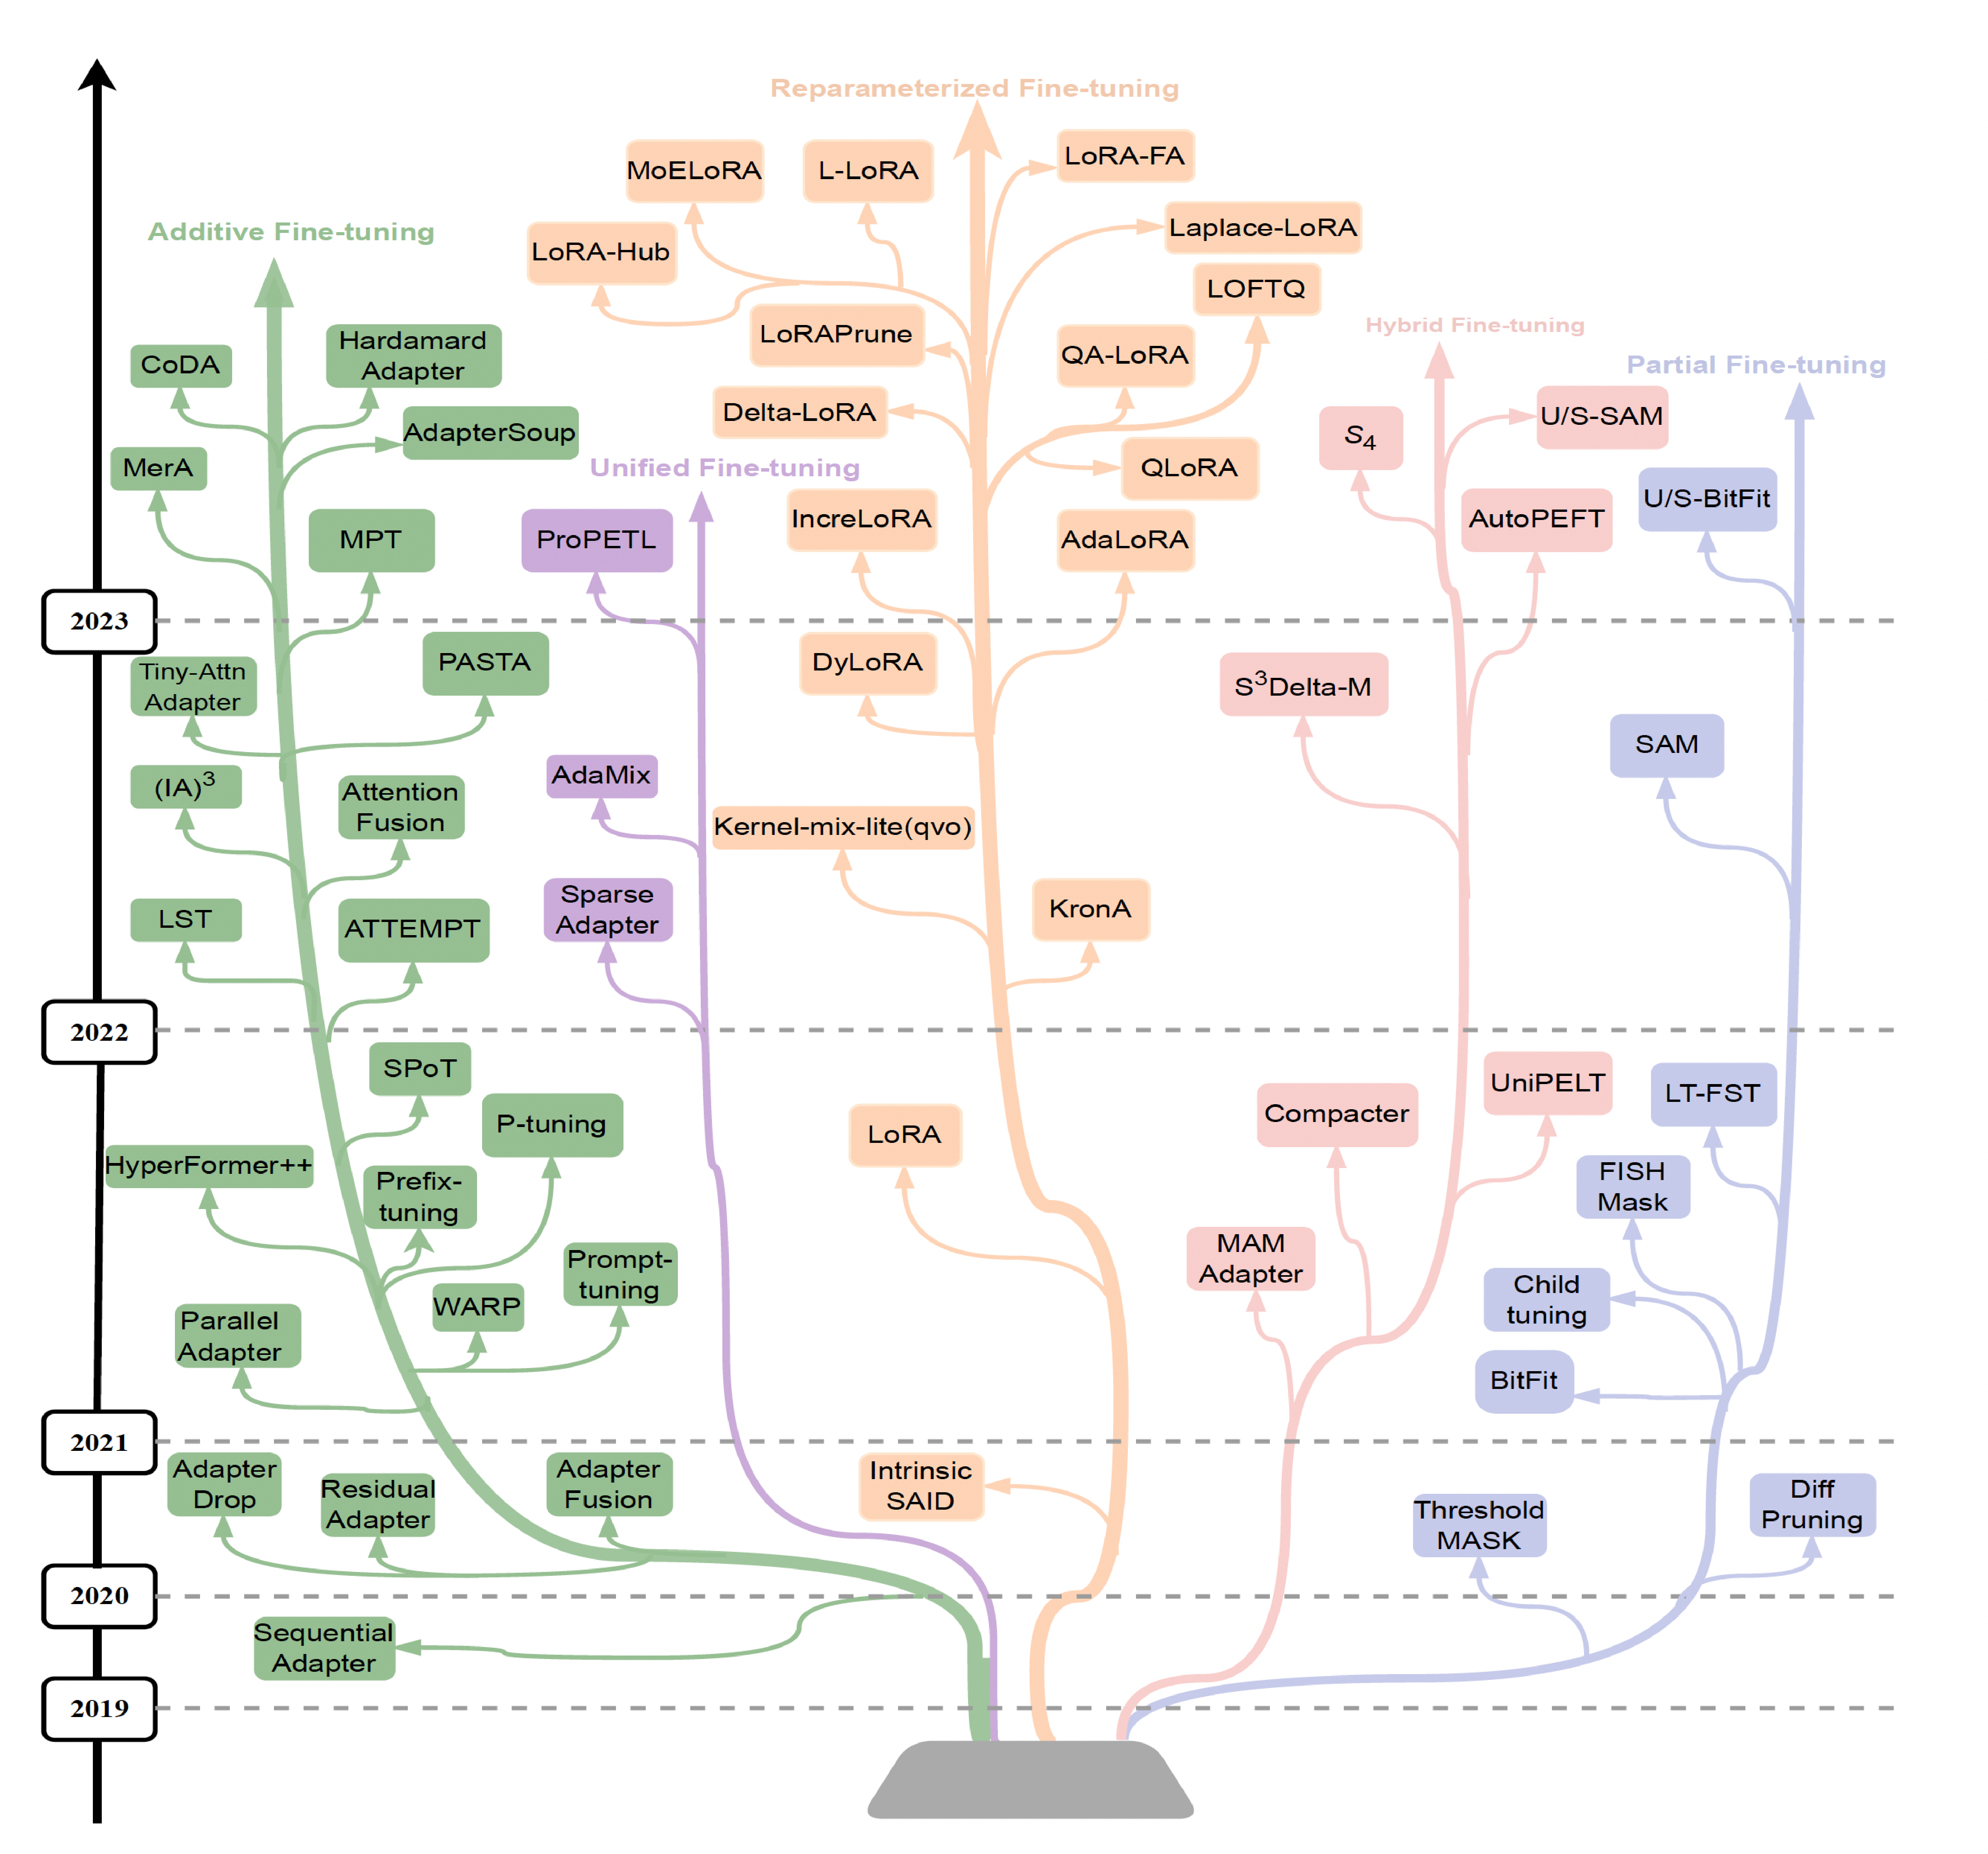
\includegraphics[width=0.9\linewidth]{results/PEFT-diagram.pdf}
	\caption{\textbf{The recent evolutionary progression of PEFT methods}, with models on the same branch sharing common features. The vertical alignment of the models indicates the timeline of their release dates \cite{Xu2023}.}
	\label{fig:PEFT-diagram}
\end{figure}


Another option is hybrid fine-tuning which combines various PEFT methods such as adapter, prefix-tuning, and LoRA to enhance performance by leveraging their strengths and mitigating weaknesses. This approach can be classified into Manual Combination and Automatic Combination. Manual Combination involves designing the combination of methods, while Automatic Combination uses structure search to incorporate these methods, requiring more time and cost \cite{mao2021unipelt, zhou2023autopeft}.

In our paper, we will explore the performance of different PEFT methods on various NLP tasks, such as machine translation and classification tasks. We will compare the performance of these methods with traditional fine-tuning and evaluate their efficiency in terms of computational resources.

\section*{Methods}

    \subsection*{Datasets and tasks}

    We explored two distinct task types: \textbf{generation} and \textbf{classification}. For text generation, we selected the Machine Translation task from \textbf{Slobench}, which evaluates the effectiveness of automatically translating Slovene to English. Additionaly, we also included various tasks from the Slovene SuperGLUE benchmark (also from Slobench) which is a Slovenian adaptation of the SuperGLUE benchmark \cite{sarlin2020superglue}. The following tasks were investigated:
    
    \begin{itemize}
        \item \textbf{BoolQ:} determine whether a given passage contains the answer to a yes/no question.
        \item \textbf{CB:} determine the commitment of a statement to a specific target.
        \item \textbf{COPA:} presents a premise and requires choosing the correct alternative explanation or cause.
        % \item \textbf{MultiRC:} answering multiple-choice questions based on a given passage, with each question having multiple correct answers.
        \item \textbf{RTE:} focuses on whether the hypothesis logically follows from the premise, often categorized as entailment and not\_entailment.
        % \item \textbf{WSC:} test machines' understanding of pronouns and their antecedents in a sentence.
     \end{itemize}
     
    \subsection*{Pretrained models}
    Based on the selected tasks, we were restricted to using models pre-trained on Slovenian data. For classification, the following models were chosen:
    
    \begin{itemize}
        \item \textbf{EMBEDDIA/sloberta:} A monolingual Slovene BERT-like model.
        \item \textbf{EMBEDDIA/crosloengual-bert:} A trilingual mo\-del, using bert-base architecture, trained on Croatian, Slovenian, and English corpora. We opted for this model due to its potential for good performance, since it is already trained on Slovenian corpora.
        \item \textbf{FacebookAI/xlm-roberta-base:} A multilingual version of RoBERTa, pre-trained on dataset containing 100 languages, including Slovene.
    \end{itemize}


    For the generation task, we needed a model designed for translation, so we used the \textbf{OPUS-MT model} \cite{huggingfaceHelsinkiNLPopusmtslaenHugging}. This model, designed for translating Slavic languages to English, is freely available and was developed by the Language Technology Research Group at the University of Helsinki.

    \subsection*{PEFT approaches}
    
    We inspected several parameter-efficient fine-tuning (PEFT) approaches available through the Hugging Face library and selected three commonly used and well-researched techniques that have demonstrated strong results in previous studies.
    
    \begin{itemize}
        \item \textbf{Prompt-Tuning:} Fine-tunes a small set of task-specific tokens appended to the input without altering the original model parameters.
        \item \textbf{LoRA:} Modifies the weight matrices of a model by applying low-rank updates, preserving the original parameters while adapting to new tasks.
        \item \textbf{LoHa:} Approximates the large weight matrix with more low-rank matrices and combines them with the Hadamard product.
     \end{itemize}
    
    \subsection*{Metrics}
    In order to evaluate the trained models, we used the metrics Accuracy, F1 score and BLEU score.

    \subsubsection*{Accuracy and F1 score}
        
        The classification tasks were evaluated based on accuracy and F1 score. Accuracy measures the proportion of correct predictions, while the F1 score combines precision and recall to account for both false positives and false negatives and is especially useful for imbalanced datasets.

    \subsubsection*{BLEU score}

    For the evaluation of the generated text from the translation task, we used the BLEU (Bilingual Evaluation Understudy) score. This metric measures the accuracy of the translated text by comparing it to a reference translation. Higher BLEU scores signify closer resemblance to the ground truth, indicating higher quality in the translation.

    \subsubsection*{GPU RAM Usage}

    To evaluate the computational resources required for tuning our models, we measured the RAM usage on the L4 GPU by recording its peak during training.

\section*{Results}
Below, the results of our work will be presented, in terms of computational resources required to fine tune the models and their performance on specific tasks.

\subsection*{Generative task}

\subsubsection*{Machine Translation}

Our first task involved translating English to Slovene using a subset of 5000 translations from the dataset RSDO4 en-sl parallel corpus \cite{huggingfaceCjvtrsdo4_en_slDatasets}. With the given dataset, we fine-tuned the opus-mt-sla-en model. 

The data presented in Figure \ref{fig:machine_translation_bleu} indicates that parameter-efficient fine-tuning techniques (LoRA, LoHA) resulted in only a slight reduction in BLEU scores compared to the fully fine-tuned model. This minor difference might be because the fully fine-tuned model can handle a diverse dataset more effectively. Parameter-efficient methods, though resource efficient, might not incorporate all necessary adjustments, especially for low resource languages, as shown in the study by Su et al. \cite{su2024unlocking}. Additionally, while both LoRa and LoHa methods had similar performance outcomes, GPU consumption was significantly higher with LoRa, suggesting that LoHa may be more advantageous when it comes to saving computer resources in this instance.

The prompt-tuning method was also implemented, however it resulted in a BLEU score of 0.004, suggesting issues with the code. Therefore, we did not include it in the evaluation. We also submitted the LoRa fine-tuned model to Slobench, the results are presented in table \ref{table:slobench_results}. 

\begin{figure}[ht]\centering
	\includegraphics[width=\linewidth]{results/machine_translation/translation_metrics.pdf}
	\caption{\textbf{BLEU score (a) and GPU memory (b) usage on machine translation task} for different parameter-efficient fine-tuning techniques.}
	\label{fig:machine_translation_bleu}
\end{figure}

\begin{table}[H]
\begin{center}
\begin{tabular}{|*{1}{>{\centering\arraybackslash}m{0.8cm}}|*{1}{>{\centering\arraybackslash}m{0.8cm}}|*{1}{>{\centering\arraybackslash}m{1.2cm}}|*{1}{>{\centering\arraybackslash}m{0.9cm}}|*{1}{>{\centering\arraybackslash}m{1cm}}|*{1}{>{\centering\arraybackslash}m{1cm}}|}
\hline
BERT score &BLEU avg &METEOR avg &CHRF avg &BLEU corpus &CHRF corpus\\
\hline
0.933 & 0.221 & 0.568 &  0.548 & 0.259 & 0.548\\
\hline

\end{tabular}
\end{center}
\caption{Slobench results on LoRa fine-tuned translation model.}
\label{table:slobench_results}
\end{table}


\subsection*{Classification tasks}
As already mentioned, we focused on 4 classification tasks from Slovene SuperGLUE dataset. We   used different PEFT approaches in order to adapt the pre-trained models (Sloberta, CroSloeEngual model, and XLM Roberta) to each specific task. Then we observed their performance on the evaluation parts of the datasets.


\subsubsection*{COPA}

We were unable to evaluate the performance of prompt-tuning for the COPA task, as multiple-choice tasks are currently not supported by Hugging Face library (issues with differences in tensor sizes).

For other methods, we evaluated the performance (F1 score) and the computational resource usage (GPU memory) of PEFT methods on our pre-trained models (Figure \ref{fig:copa_scores}). All models performed similarly on the task. For the CroSloEngual model, the LoHa and LoRa methods both outperformed simple fine-tuning, with LoHa nearly doubling the F1 score. For the Sloberta and XLM Roberta models, both PEFT methods outperformed fine-tuning, with LoRa leading in both cases. Additionally, there was a significant reduction in GPU usage, with PEFT methods requiring substantially less memory. Notably, PEFT tuning on XLM Roberta required four times less GPU memory. From this, we can conclude that PEFT methods are more efficient in terms of computational resources and can achieve similar or better performance than full fine-tuning for the COPA task. 

\begin{figure}[ht]\centering
	\includegraphics[width=\linewidth]{results/superglue/COPA.pdf}
	\caption{\textbf{F1 score (a) and GPU memory (b) usage on COPA task} for different parameter-efficient fine-tuning techniques.}
	\label{fig:copa_scores}
\end{figure}

\subsubsection*{CB}

For the CB task, we observed a different trend in performance (Figure \ref{fig:cb_scores}). In almost all cases, except for the LoHa method on the Sloberta model, the F1 score dropped significantly compared to regular fine-tuning. This might be due to the complexity of the task, which requires a more thorough understanding of the text, and key parameters might not have been tuned by the PEFT methods. However, GPU memory usage was significantly lower for all PEFT methods, with LoHa requiring the least memory. The superior performance of LoHa on the Sloberta model could be attributed to the specific architecture or parameter settings of the Sloberta model, which might align better with the LoHa method's optimization process. This indicates that while PEFT methods are more efficient in terms of computational resources, they might not be as effective as full fine-tuning for the CB task.

\begin{figure}[ht]\centering
	\includegraphics[width=\linewidth]{results/superglue/CB.pdf}
	\caption{\textbf{F1 score (a) and GPU memory usage (b) on CB task} for different parameter-efficient fine-tuning techniques.}
	\label{fig:cb_scores}
\end{figure}

\subsubsection*{BoolQ}

Here, we observed a trend similar to that seen with the COPA task (Figure \ref{fig:boolq_scores}). In most cases, PEFT methods outperformed full fine-tuning, except for LoRa and prompt-tuning on the CroSloEngual model, where the result was slightly worse. GPU memory usage was significantly lower for all PEFT methods. Notably, for the Sloberta model, LoHa required four times less memory than full fine-tuning and three times less than LoRa, while achieving the highest F1 score. This indicates that PEFT methods are more efficient in terms of computational resources and can achieve similar or better performance than full fine-tuning for the BoolQ task.

\begin{figure}[ht]\centering
	\includegraphics[width=\linewidth]{results/superglue/BoolQ.pdf}
	\caption{\textbf{F1 score (a) and GPU memory usage (b) on BoolQ task} for different parameter-efficient fine-tuning techniques.}
	\label{fig:boolq_scores}
\end{figure}

\subsubsection*{RTE}

For this task, we observed a new trend in performance (Figure \ref{fig:rte_scores}). In most cases, PEFT methods performed slightly worse than full fine-tuning, except for LoRa on the XLM Roberta model. This could be due to the specific architecture of XLM Roberta aligning better with LoRa's optimization process for this task. Another notable observation is that prompt tuning did not perform well on this task with the XLM Roberta model, possibly due to the complexity of the task requiring more nuanced parameter adjustments. The trend of lower GPU memory usage for PEFT methods continued, with LoHa requiring the least memory in most cases. This indicates that while PEFT methods are more efficient in terms of computational resources, they might not be as effective as full fine-tuning for the RTE task, potentially due to the task's complexity demanding more comprehensive fine-tuning.

\begin{figure}[ht]\centering
	\includegraphics[width=\linewidth]{results/superglue/RTE.pdf}
	\caption{\textbf{F1 score (a) and GPU memory usage (b) on RTE task} for different parameter-efficient fine-tuning techniques.}
	\label{fig:rte_scores}
\end{figure}

% Up to this point, we tried to fine tune some models on different tasks from the dataset. The results are shown in tables \ref{table:boolq_performance}, \ref{table:cb_performance} and \ref{table:copa_performance}. During the process of training and fine tuning, we ran into some problems, as the models achieved very bad performance in some cases. Despite thorough debugging and testing of our implementations, we are still not sure if there is a bug in our code or if the models really just struggle with these tasks.

% Use the results section to present the final results of your work. Present the results in a objective and scientific fashion. Use visualisations to convey your results in a clear and efficient manner. When comparing results between various techniques use appropriate statistical methodology.



%------------------------------------------------

\section*{Discussion}

During the adaptation of the models for different tasks, we reached some interesting findings. We can conclude that PEFT methods really are efficient, as they drastically reduce the need for computational resources, when used for adapting large pretrained models.
In addition to that, they are able to match or even outperform fully fine-tuned models in terms of F1 scores. However there can be some exceptions, as observed with the CB task, where PEFT methods failed to match the performance of traditional fine-tuning. We suspect that the complexity of the task, poses a significant challenge and since PEFT methods only adjust a small subset of the model's parameters, this limited scope may be insufficient for capturing the depth of understanding needed to perform well on such task.

Another instance where the performance of the LoRA and LoHa techniques fell short compared to the fully fine-tuned model was noted in the translation task. As mentioned in the results section this could be due to slovenian being a low resource language, an issue that has been identified in other studies as well.

In the future, we could include some larger pre-trained models, which could potentially yield better results. With increased numbers of parameters in those models, we would be able to illustrate the efficiency of PEFT methods even better.
Given additional time, we would prioritize the implementation of the remaining two tasks from the Slovene SuperGLUE dataset. This way we would be able to publicly submit the test set results to Slobench and gain insight in how well our models really performed in comparison to other submissions.

% Use the Discussion section to objectively evaluate your work, do not just put praise on everything you did, be critical and exposes flaws and weaknesses of your solution. You can also explain what you would do differently if you would be able to start again and what upgrades could be done on the project in the future.


%------------------------------------------------

% \section*{Acknowledgments}
% TODO
% Here you can thank other persons (advisors, colleagues ...) that contributed to the successful completion of your project.


%----------------------------------------------------------------------------------------
%	REFERENCE LIST
%----------------------------------------------------------------------------------------
\bibliographystyle{unsrt}
\bibliography{report}


\end{document}